\section{Introduction}
\label{sec:intro}

Visual-Based Localization (VBL) is a central topic in robotics and computer vision applications~\cite{Piasco2017}. It consists in retrieving the location of a visual query according to a known absolute reference. VBL is used in many applications such as autonomous driving, augmented reality, robot navigation or SLAM loop closing. In this paper, we address VBL as an image retrieval problem where an input image is compared to a reference pool of localized images. This image-retrieval-like problem is two-step: descriptor computation for both the query and the reference images and similarity association across the descriptors. Since the reference images are associated to a location, by ranking images according to their similarity scores we obtain an approximate location for the query. Numerous works have introduced image descriptors well suited for image retrieval for localization~\cite{Arandjelovic2017,Kim2017a,Gordo2017,Radenovic2017,Liu2018}. We present in figure~\ref{fig:our_method_deployment} our learned descriptor and the entire image localization pipeline. The final localization obtain by such system can be used as it or as initialization for pose refinement method~\cite{Sattler2017a, Sarlin2018a, Piasco2019a}. In this paper, we focus on building a discriminative image descriptor for initial pose localization by image retrieval so we do not investigate refinement pose method.

One of the main challenges of image-based localization remains the mapping of images acquired under changing conditions: cross-season images matching~\cite{Naseer2017a}, long-term localization~\cite{Toft2018}, day to night place recognition~\cite{Torii2015}, etc. Recent approaches use complementary information in order to address these visually challenging localization scenarios (geometric information through point cloud~\cite{Sattler2018,Schonberger2018} or depth maps~\cite{Christie2016}, semantic information~\cite{Ardeshir2014,Christie2016,Naseer2017a}). However geometric or semantic information are not always available or can be costly to obtain, especially in robotic or mobile applications when the sensor or the computational load on the system is limited.

In this paper, we propose a image descriptor capables of reproducing the underlying scene geometry from an monocular image, in order to deal with challenging outdoor large-scale image-based localization scenarios. We introduce dense geometric information as side training objectif to make our new descriptor robust to visual changes that occur between images taken at different times. Once trained, our system can be used on monocular images only to construct a expressive descriptor for image retrieval. This kind of system design is also known as side information learning~\cite{Hoffman2016}, as it uses geometric and radiometric information only during the training step and pure radiometric data for the image localization. 

\begin{figure}
	\center
	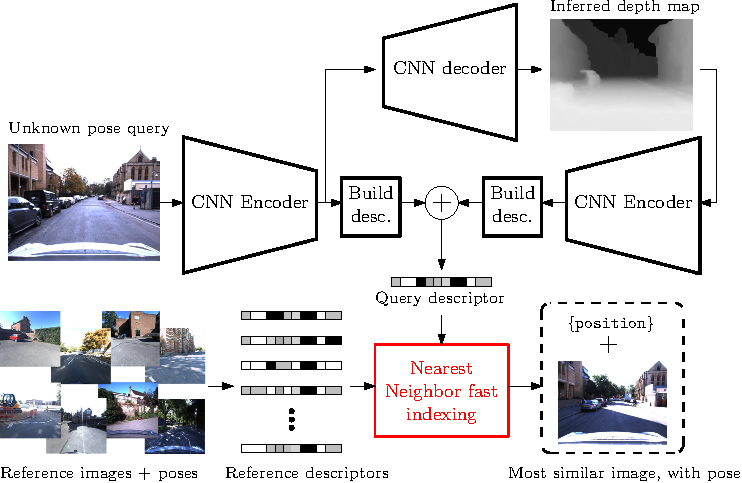
\includegraphics[width=\linewidth]{intro/visual_abstract}
	\caption{\label{fig:our_method_deployment} \textbf{Our method at test time:} we rely \textit{only on radiometric data} (= monocular images) to build low dimensional global image features used for localization. The reconstructed depth map used for image description make our method more robust to visual changes that occurs in long-term localization scenarios.}
\end{figure}

The paper is organized as follows. In section~\ref{sec:related_work}, we first revisit recent works related to our method, including:~state of the art image descriptors for large scale outdoor localization, method for localization in changing environment, side information learning approaches and depth from monocular for localization. In section~\ref{sec:method}, we describe in detail our new image descriptor trained with side depth information. In section~\ref{sec:impl_details} we give insight on our implementation and the dataset we used and we illustrate the effectiveness of the proposed method on six challenging scenarios in section~\ref{sec:experiments}. We discuss in section~\ref{sec:chall_loc} about the challenging night to day localization scenario and in section~\ref{sec:modality_ref} we present a variation of our method using dense object reflectance map instead of depth maps. Section~\ref{sec:conclusion} finally concludes the paper.

We extend the method proposed in~\cite{Piasco2019} with three original contribution: we report results on another 3 challenging scenarios from a different dataset that the one used to train the system, we investigate the impact of fine tuning the method for night to day localization and by we expend the proposed method to another side modality, object reflectance, instead of depth map.

